\documentclass{article}

	\usepackage[english]{babel}
	\usepackage{xspace}
	\usepackage{graphicx}
	\usepackage{hyperref}

	\newcommand{\latex}{\LaTeX\xspace}
	\newcommand{\email}[1]{\texttt{#1}}

\begin{document}

\title{
	A Guide to \latex Editing in Visual Studio Code\\
	\large Written in \latex with Visual Studio Code
}
\author{
	Dan Arad\\
	\email{arda@bgu.ac.il}
}
\maketitle

\section{Introduction}
This guide's purpose is to help setup a comfortable and efficient editing of \latex documents using Visual Studio Code\footnotemark[1] (also known as VSCode). This also includes the ability to easily work with git version control, and keep generated files out of the way.\\
VSCode is a free open source powerful light-weight editor developed and maintained by Microsoft. The editor boasts many extensions and built-in git support, and is widely used. Among its many extension, there is one called \emph{\latex Workshop}\footnotemark[2].\\
To me VSCode is the first choice for editing any kind of code, and for that reason I chose to see how well it will preform as a \latex editor. I was not dissapointed with the result.

\footnotetext[1]{Homepage: https://code.visualstudio.com/}
\footnotetext[2]{Extension Site: https://marketplace.visualstudio.com/items?itemName=James-Yu.latex-workshop}
\footnotetext[3]{The Guide: https://dev.to/nickymarino/lets-use-latex}

\section{Basic Setup}
For the basic setup of VSCode with \latex I used Nicky Marino's guide\footnotemark[3], and this entire section is based on it.\\
At the conclusion of this basic setup, you will have everything you need to get going:
\begin{itemize}
	\item{Syntax highlighting for \latex}
	\item{Preview option that is updated either manualy, on save or on change of the document}
	\item{An outline of your \latex document}
	\item{Error and warning pane}
\end{itemize}
Figure \ref{fig:vscode_with_latex_highlights} displays the outcome and the different components.
\begin{figure}
	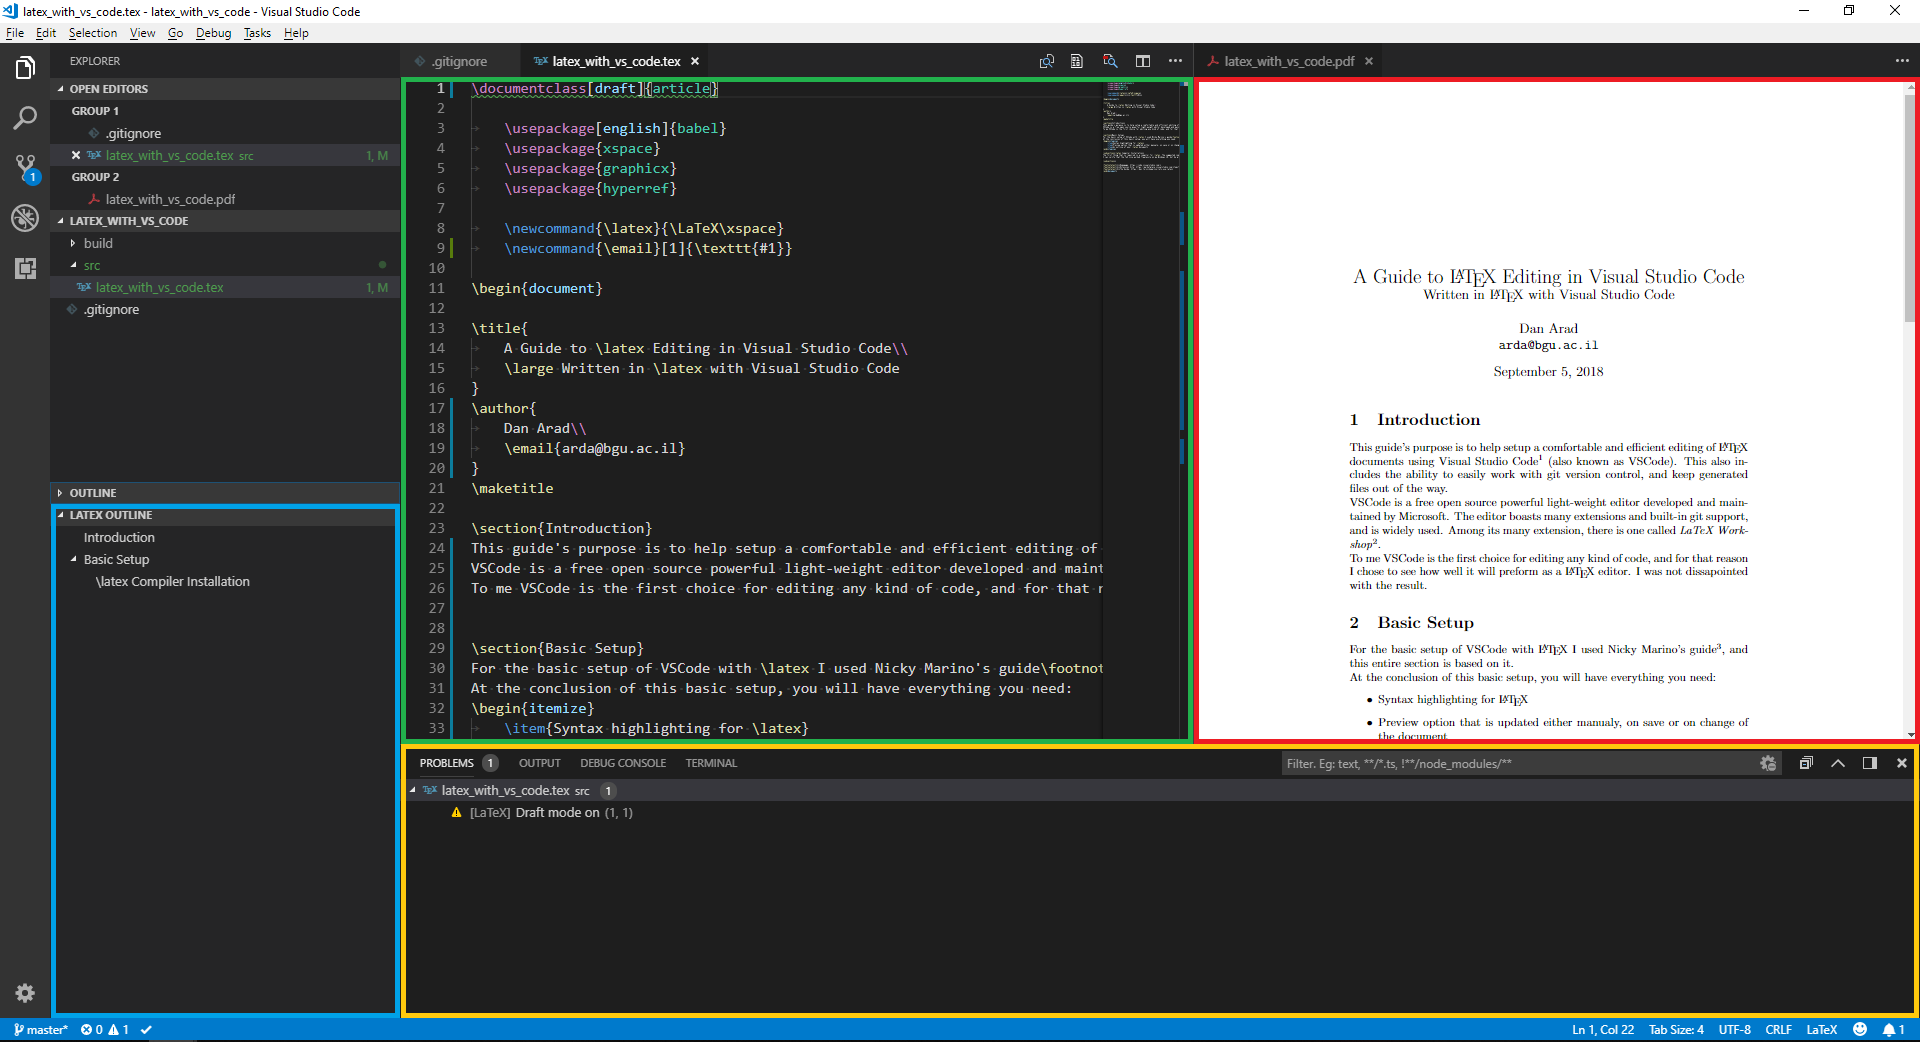
\includegraphics[width=\linewidth]{../resources/vscode_with_latex_highlights.png}
	\caption{Green: Code Highlighting, Red: Preview, Blue: Outline, Yellow: Errors and Warnings}
	\label{fig:vscode_with_latex_highlights}
\end{figure}

\subsection{\latex Compiler Installation}
The first thing that is required is a compiler for \latex. The suggested compiler is \emph{TeX Live} for Windows and Linux, and \emph{MacTex} for MacOS.\\
I can verify that the TeX Live worked flawlessly on my Windows 10, but be prepared - It's a very long installation.

\subsection{VScode and \latex Workshop Installation}
If you don't have VSCode installed, install it from the official website\footnotemark[1].\\
Then, in VSCode go to the extension marketplace by clicking the button marked in figure \ref{fig:vscode_marketplace}, or by using the shortcut Ctrl+Shift+X. Search for \latex Workshop, click install, and when finished, click reload.\\
After the editor reloads, you should be able to use all the previously discussed functionalities.
\begin{figure}
	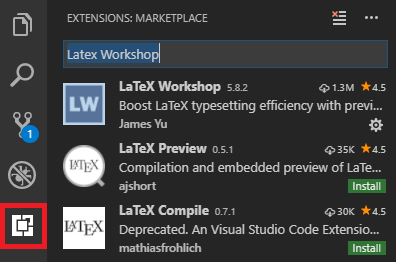
\includegraphics[width=\linewidth]{../resources/vscode_marketplace.png}
	\caption{The marketplace is marked in red}
	\label{fig:vscode_marketplace}
\end{figure}


\section{Additional Know-How}
I will not go in depth explaining the features of VSCode, but I do find it important to talk about the issue of extension commands and settings.

\subsection{Commands}
In VSCode, each extension may define commands, that can be run by the user. To run a command use the Ctrl+Shift+p shortcut that opens context menu with all available commands. This is highlighted in figure \ref{fig:command_menu}.\\
\latex Workshop defines several such commands. The most useful I found are \emph{LaTeX Workshop: Build LaTeX project}, which can also be activated using Ctrl+Alt+B, \emph{laTeX Workshop: Clean up auxiliary files} and \emph{LaTeX Workshop: View LaTeX PDF file in VSCode tab}, that can also be triggered by using the button indicated in figure \ref{fig:command_menu}.
\begin{figure}
	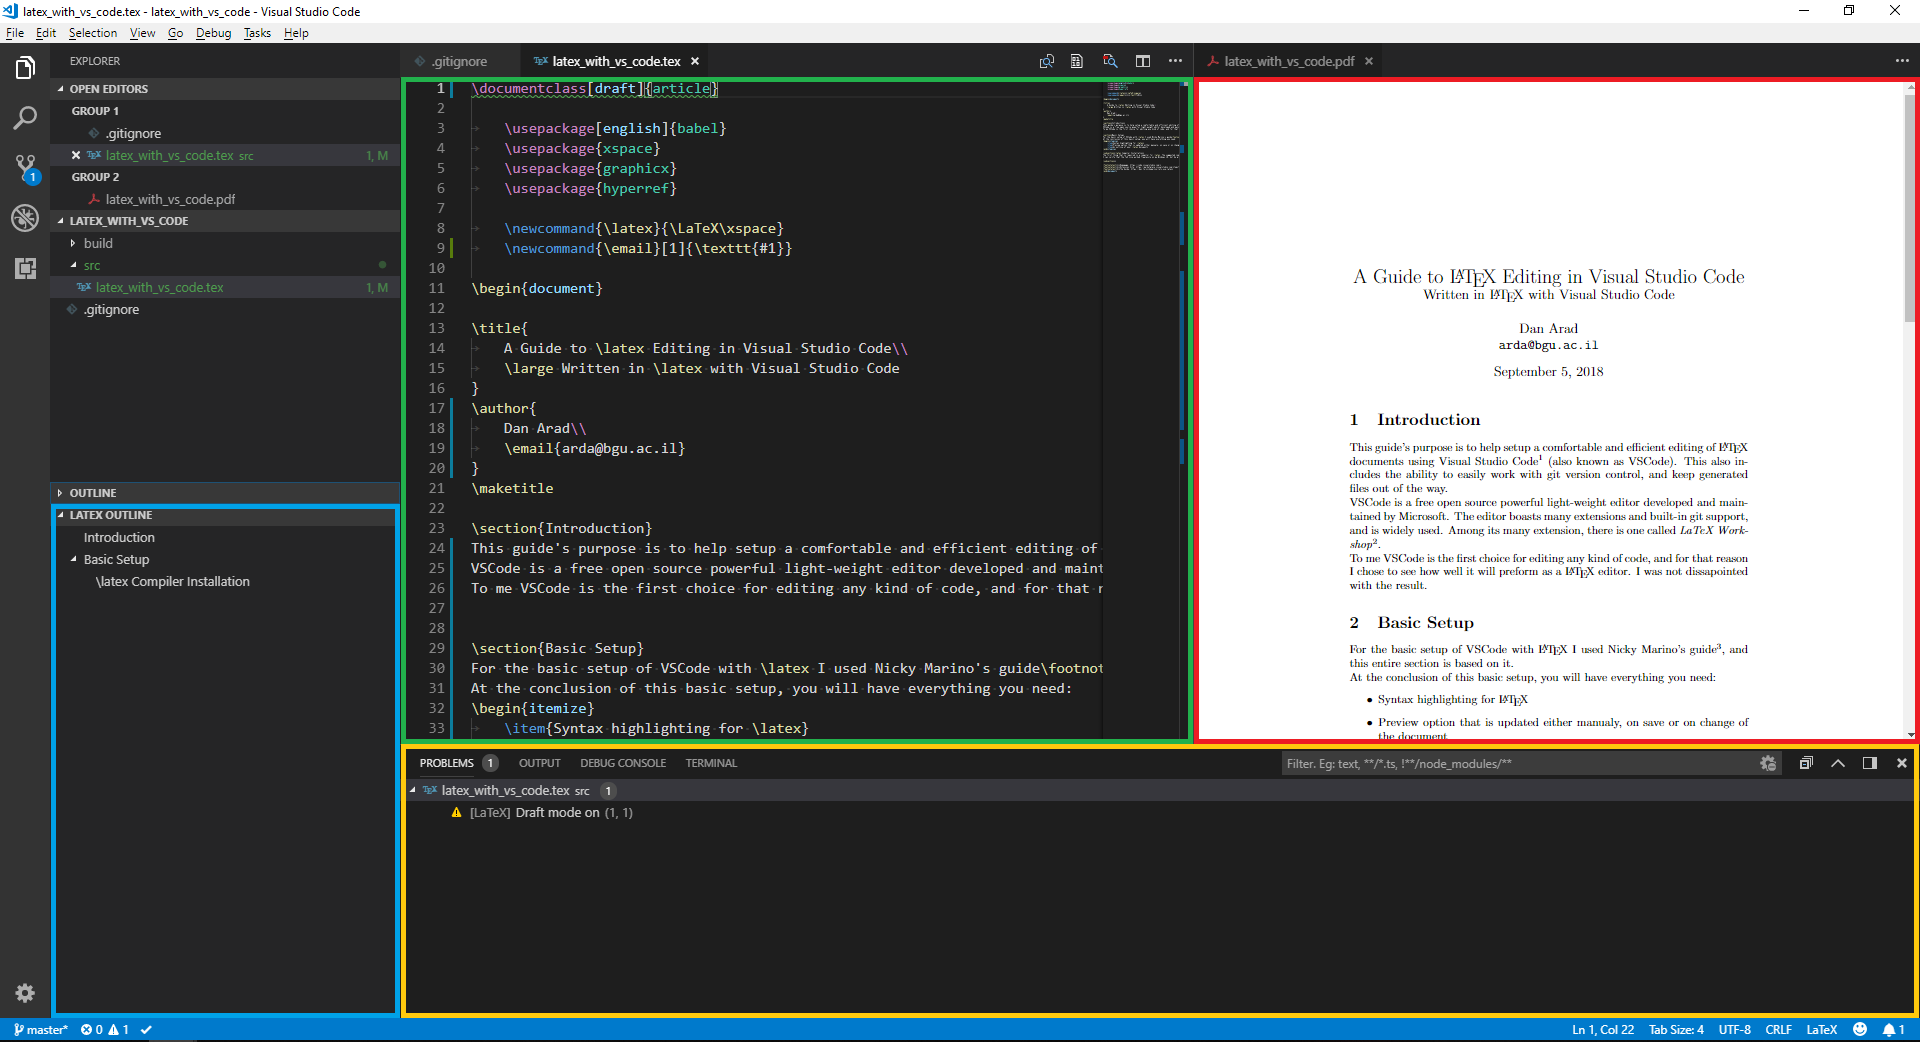
\includegraphics[width=\linewidth]{../resources/vscode_with_latex_highlights.png}
	\caption{Green: Code Highlighting, Red: Preview, Blue: Outline, Yellow: Errors and Warnings}
	\label{fig:command_menu}
\end{figure}

\subsection{Settings}
Each extension also has its own settings that are controlled through the Settings window of VSCode. The settings are grouped by category, and each extension has its own group.\\
To open the settings window go to File -> Preferences -> Settings, or use the Ctrl+, shortcut.
\latex Workshop

\section{Seperating Sources from Outputs}
I was very pleased when I finished the installations and everything worked smoothly, but I did have one reservation. Every time there was a new build (which to me is configured to happen every )

\end{document}